\subsection{Struttura di Clarke per la selezione}
La struttura di Clarke per la selezione è succinta teoricamente, ma in pratica
è raramente utilizzata come descritta perché la sua implementazione è molto
complessa.
L'obiettivo è, dato un vettore $\mathbf{b}$ di valori binari fissato, calcolare
la funzione di selezione
$$
	\mathbf{select_b}(k) = \text{ posizione del } k-\text{esimo } 1
$$
La struttura di Clarke utilizza dei \textit{livelli}, simili a quelli utilizzati
dalla struttura di Jacobson.

\subsubsection{Primo livello}
Il primo livello della struttura di Clarke è un insieme
di valori che rappresentano le posizioni degli $1$ di ordinalità multipla di
$\log_2(n) \cdot \log_2(\log_2(n))$, ossia
$$
	P_i =  \mathbf{select_b}(i \cdot \log_2(n) \cdot \log_2(\log_2(n)))
$$
ossia la posizione del $(i \cdot \log_2(n) \cdot \log_2(\log_2(n)))$-esimo $1$.

\paragraph{Memoria}
La grandezza di questa famiglia, ossia il numero di $P_i$, dipende dal
numero di $i$ che ci sono in $\mathbf{b}$, ma nel caso peggiore, il vettore
è composto unicamente da $1$ e vi saranno $\frac{n}{\log_2(n) \cdot \log_2(\log_2(n))}$ membri.
Ad ognuno di essi va associato un elemento, il quale richiede $\log_2(n)$ bit;
in totale, questo livello occupa
$$
	\frac{n}{\log_2(n) \cdot \log_2(\log_2(n))} \cdot \log_2(n) = o(n) \text{ bit}
$$

\subsubsection{Secondo livello}
Per le posizioni che non sono multiple di $\log_2(n) \cdot \log_2(\log_2(n))$ si utilizza
un secondo livello, che è costruito differentemente in base ad un indice calcolato
per ogni $P_i$:

$$
	\forall i ~ r_i = P_{i + 1} - P_i
$$
che rappresenta la distanza fra l'$(i \cdot \log_2(n) \cdot \log_2(\log_2(n)))$-esimo $1$
e il $((i+1) \cdot \log_2(n) \cdot \log_2(\log_2(n)))$-esimo. Questo
valore, $r_i$, sarà esattamente uguale a $\log_2(n) \cdot \log_2(\log_2(n))$ se e solo se
tra $P_{i}$ e $P_{i+1}$ ci sono unicamente $1$, e sarà maggiore se invece le
due posizioni sono più lontane.
% @TODO: serve un esempio, non si capisce bene.
I due casi che si considerano dipendono dal valore di $r_i$.

\paragraph{Caso sparso}
Se $r_i \geq (\log_2(n) \cdot \log_2(\log_2(n)))^2$, significa che in $\mathbf{b}$ ci
sono molti $0$ tra gli $1$ contenuti nelle posizioni tra $P_{i}$ e $P_{i+1}$; in questo caso
definiamo $S_i$ come la lista esplicita delle posizioni di tutti gli $1$
in $\mathbf{b}$ tra le due posizioni rappresentate come differenza tra $P_i$.

In questo caso, gli $S_i$ costruiti sono esattamente $\log_2(n)\cdot \log_2(\log_2(n))$,
in quanto stiamo contando gli $1$ in $\mathbf{b}$ tra il $(i \cdot \log_2(n) \cdot \log_2(\log_2(n))$-esimo
$1$ e il $((i+1) \cdot \log_2(n) \cdot \log_2(\log_2(n))$-esimo $1$, e ad ognuno
di essi si associa un numero che in grandezza è minore o uguale a
$\log_2(r_i)$, concludendo che per memorizzare un $S_i$ sono necessari
\begin{align*}
	\log_2(n)\cdot \log_2(\log_2(n)) \cdot \log_2(r_i) & = \frac{(\log_2(n)\cdot \log_2(\log_2(n)))^2}{\log_2(n)\cdot \log_2(\log_2(n))} \cdot \log_2(r_i) \\
	                                                   & \leq \frac{r_i}{\log_2(n)\cdot \log_2(\log_2(n))} \cdot \log_2(r_i)                               \\
	                                                   & \leq \frac{r_i}{\log_2(n)\cdot \log_2(\log_2(n))} \cdot \log_2(n)                                 \\
	                                                   & \leq \frac{r_i}{\log_2(\log_2(n))}                                                                \\
	                                                   & \leq \frac{n}{\log_2(\log_2(n))}   = o(n) \text{ bit}
\end{align*}

\paragraph{Caso denso}
Se $r_i \le (\log_2(n) \cdot \log_2(\log_2(n)))^2$, si memorizzano gli $1$
multipli di $\log_2(r_i)\log_2(\log_2(n))$, ossia partendo dalla posizione $P_i$ si salvano le
posizioni degli $j \cdot \log_2(r_i)\log_2(\log_2(n))$-esimi $1$ come differenze da $P_i$, ossia
$$
	S^i_j = \mathbf{select_b}(j \cdot \log_2(r_i)\log_2(\log_2(n))) - P_i
$$

In questo caso, gli $1$ memorizzati sono $\frac{\log_2(n)\cdot \log_2(\log_2(n))}{\log_2(r_i)\cdot \log_2(\log_2(n))}$.
Ad ognuno di questi si associa un valore in grandezza $\log_2(r_i)$, quindi lo spazio utilizzato
per memorizzare tutti i valori $S^i_j$ sono
$$
	\frac{\log_2(n)\cdot \log_2(\log_2(n))}{\log_2(r_i)\cdot \log_2(\log_2(n))} \log_2(r_i) =
	\frac{\log_2(n)\cdot \log_2(\log_2(n))}{\log_2(\log_2(n))} \leq \frac{r_i}{\log_2(\log_2(n))}
	\leq \frac{n}{\log_2(\log_2(n))} = o(n) \text{ bit}
$$


\subsubsection{Terzo livello}
Se nel secondo livello ci si trova nel caso denso, si utilizza un terzo livello.
Questo livello viene utilizzato esclusivamente per gli $1$ le cui posizioni non sono state
salvate nel secondo livello nel caso denso; pertanto, l'assunto è che
$$
	r_i < (\log_2(n) \log_2(\log_2(n)))^2
$$
Per ognuna di queste posizioni calcoliamo la differenza tra $S^i_j$:
$$
	\forall j ~~ \bar{r}^i_j = S^i_{j+1} - S^i_j
$$
Come nel caso precedente, abbiamo due possibilità in base al valore di $\bar{r}^i_j$, il quale
gode comunque della proprietà
$$
	\forall i, j ~~  \bar{r}^i_j \geq \log_2(r_i) \log_2(\log_2(n))
$$
\paragraph{Caso sparso}
Nel caso in cui $\bar{r}^i_j \geq \log_2(\bar{r}^i_j) \log_2(r_i) \log_2(\log_2(n))^2$,
si memorizzano esplicitamente tutte le posizioni degli $1$ tra $S^i_j$ e $S^i_{j+1}$
con dei valori $T^i_{j,k}$ come differenze tra $S^i_j$. In questo caso,
il consumo di memoria è
$$
	(\log_2(r_i)\cdot \log_2(\log_2(n)) \cdot \log_2(\bar{r}^i_j) \leq
	\frac{\log_2(r_i) \cdot \log_2(\log_2(n))^2 \log_2(\bar{r}^i_j)}{\log_2(\log_2(n))}
	\leq \frac{\bar{r}^i_j}{\log_2(\log_2(n))} = o(n) \text{ bit}
$$
\paragraph{Caso denso}
Nel caso in cui $\bar{r}^i_j \le \log_2(\bar{r}^i_j) \log_2(r_i) \log_2(\log_2(n))^2$,
significa che ci sono pochi $0$ tra $S^i_j$ e $S^i_{j+1}$ e
si utilizza il four-russians trick. Inizialmente osserviamo quanto segue.
\begin{oss}
	\begin{align*}
		\log_2(\bar{r}^i_j) \leq \log_2(r_i) & \leq \log_2(\log_2(n)\cdot \log_2(\log_2(n)))^2     \\
		                                     & = 2 \log_2(\log_2(n)) + 2 \log_2(\log_2(\log_2(n))) \\
		                                     & \leq 4 \log_2(\log_2(n))
	\end{align*}
\end{oss}
\begin{oss}
	$$
		\bar{r}^i_j < \log_2(\bar{r}^i_j) \cdot \log_2(r_i) \cdot (\log_2(\log_2(n))^2
		\leq 16(\log_2\log_2(n))^4
	$$
\end{oss}
Lo spazio necessario per utilizzare il four-russians trick è quanto segue.
Servono $2^{\bar{r}^i_j}$ enumerazioni di `sottovettori',
ossia la dimensione tra $S^i_j$ e $S^i_{j+1}$,
che è la parte che va memorizzata esplicitamente; per ognuna di queste
enumerazioni è necessario salvare la posizione di $\bar{r}^i_j$ $1$ utilizzando
memoria al massimo $\log_2(\bar{r}^i_j)$:
\begin{align*}
	2^{\bar{r}^i_j} \cdot \bar{r}^i_j \cdot \log_2(\bar{r}^i_j) & \leq
	2^{16(\log_2\log_2(n))^4} \cdot 16(\log_2\log_2(n))^4 \cdot \log_2(16(\log_2\log_2(n))^4)                                  \\
	                                                            & = 16(\log_2\log_2(n))^8 \log_2(16(\log_2\log_2(n))^4) = o(n)
\end{align*}


\subsubsection{Complessità totale in spazio}
In totale, per memorizzare $\mathbf{b}$ e i possibili tre livelli di struttura,
sono necessari $o(n)$ bit per il primo livello e, in base a come è fatto il secondo livello
$$
	\sum^{\frac{n}{\log_2(n)\cdot \log_2(\log_2(n))}} \frac{P_{i+1} - P_i}{\log_2(\log_2(n)}
	= \frac{P_n - P_0}{\log_2(\log_2(n))}
	\leq \frac{n}{\log_2(\log_2(n))} = o(n) \text{ bit}
$$
più $o(n)$ bit per il terzo livello. Quindi, la struttura di Clarke occupa
spazio $n + o(n)$ e ha tempo di accesso costante, pertanto è
una struttura \textbf{succinta}.

\begin{figure}
	\centering
	\tikzset{every picture/.style={line width=0.75pt}} %set default line width to 0.75pt

	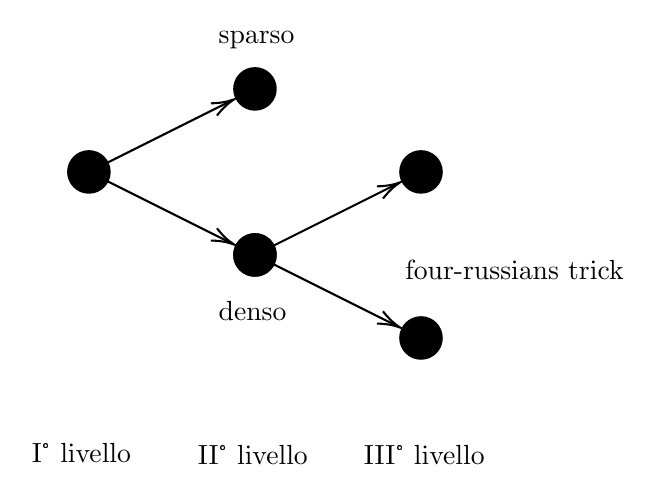
\begin{tikzpicture}[x=0.75pt,y=0.75pt,yscale=-1,xscale=1]
		\draw  [fill={rgb, 255:red, 0; green, 0; blue, 0 }  ,fill opacity=1 ] (70,101) .. controls (70,95.48) and (74.48,91) .. (80,91) .. controls (85.52,91) and (90,95.48) .. (90,101) .. controls (90,106.52) and (85.52,111) .. (80,111) .. controls (74.48,111) and (70,106.52) .. (70,101) -- cycle ;
		\draw  [fill={rgb, 255:red, 0; green, 0; blue, 0 }  ,fill opacity=1 ] (150,61) .. controls (150,55.48) and (154.48,51) .. (160,51) .. controls (165.52,51) and (170,55.48) .. (170,61) .. controls (170,66.52) and (165.52,71) .. (160,71) .. controls (154.48,71) and (150,66.52) .. (150,61) -- cycle ;
		\draw    (80,101) -- (148.21,66.89) ;
		\draw [shift={(150,66)}, rotate = 153.43] [color={rgb, 255:red, 0; green, 0; blue, 0 }  ][line width=0.75]    (10.93,-3.29) .. controls (6.95,-1.4) and (3.31,-0.3) .. (0,0) .. controls (3.31,0.3) and (6.95,1.4) .. (10.93,3.29)   ;
		\draw  [fill={rgb, 255:red, 0; green, 0; blue, 0 }  ,fill opacity=1 ] (150,141) .. controls (150,146.52) and (154.48,151) .. (160,151) .. controls (165.52,151) and (170,146.52) .. (170,141) .. controls (170,135.48) and (165.52,131) .. (160,131) .. controls (154.48,131) and (150,135.48) .. (150,141) -- cycle ;
		\draw    (80,101) -- (148.21,135.11) ;
		\draw [shift={(150,136)}, rotate = 206.57] [color={rgb, 255:red, 0; green, 0; blue, 0 }  ][line width=0.75]    (10.93,-3.29) .. controls (6.95,-1.4) and (3.31,-0.3) .. (0,0) .. controls (3.31,0.3) and (6.95,1.4) .. (10.93,3.29)   ;
		\draw  [fill={rgb, 255:red, 0; green, 0; blue, 0 }  ,fill opacity=1 ] (150,141) .. controls (150,135.48) and (154.48,131) .. (160,131) .. controls (165.52,131) and (170,135.48) .. (170,141) .. controls (170,146.52) and (165.52,151) .. (160,151) .. controls (154.48,151) and (150,146.52) .. (150,141) -- cycle ;
		\draw  [fill={rgb, 255:red, 0; green, 0; blue, 0 }  ,fill opacity=1 ] (230,101) .. controls (230,95.48) and (234.48,91) .. (240,91) .. controls (245.52,91) and (250,95.48) .. (250,101) .. controls (250,106.52) and (245.52,111) .. (240,111) .. controls (234.48,111) and (230,106.52) .. (230,101) -- cycle ;
		\draw    (160,141) -- (228.21,106.89) ;
		\draw [shift={(230,106)}, rotate = 153.43] [color={rgb, 255:red, 0; green, 0; blue, 0 }  ][line width=0.75]    (10.93,-3.29) .. controls (6.95,-1.4) and (3.31,-0.3) .. (0,0) .. controls (3.31,0.3) and (6.95,1.4) .. (10.93,3.29)   ;
		\draw  [fill={rgb, 255:red, 0; green, 0; blue, 0 }  ,fill opacity=1 ] (230,181) .. controls (230,186.52) and (234.48,191) .. (240,191) .. controls (245.52,191) and (250,186.52) .. (250,181) .. controls (250,175.48) and (245.52,171) .. (240,171) .. controls (234.48,171) and (230,175.48) .. (230,181) -- cycle ;
		\draw    (160,141) -- (228.21,175.11) ;
		\draw [shift={(230,176)}, rotate = 206.57] [color={rgb, 255:red, 0; green, 0; blue, 0 }  ][line width=0.75]    (10.93,-3.29) .. controls (6.95,-1.4) and (3.31,-0.3) .. (0,0) .. controls (3.31,0.3) and (6.95,1.4) .. (10.93,3.29)   ;

		\draw (51,230) node [anchor=north west][inner sep=0.75pt]   [align=left] {I° livello};
		\draw (131,231) node [anchor=north west][inner sep=0.75pt]   [align=left] {II° livello};
		\draw (211,231) node [anchor=north west][inner sep=0.75pt]   [align=left] {III° livello};
		\draw (141,162) node [anchor=north west][inner sep=0.75pt]   [align=left] {denso};
		\draw (141,32) node [anchor=north west][inner sep=0.75pt]   [align=left] {sparso};
		\draw (231,142) node [anchor=north west][inner sep=0.75pt]   [align=left] {four-russians trick};
	\end{tikzpicture}
	\caption{Struttura di Clarke per la selezione.}
\end{figure}
